%!TEX program = xelatex

\documentclass[11pt,titlepage]{report}
%!TEX root = main.tex

\usepackage[T1]{fontenc}
\usepackage{lmodern}
\usepackage[svgnames]{xcolor}
\usepackage{fontspec} % XeLaTeX required!
\usepackage{graphicx}
\usepackage{circuitikz}
\usepackage{tikz}
\usepackage{pifont}
\usepackage[some]{background}
\usepackage{xltxtra} 
\usepackage{setspace}
\usepackage[absolute]{textpos}
\usepackage[latin1]{inputenc}
\usepackage[english]{babel}
\usepackage{graphicx}
\usepackage{wrapfig}
\usepackage{fullpage}
\usepackage[margin=1in]{geometry}
\usepackage{float}
\usepackage{url}
\usepackage{multicol}
\usepackage{hyperref}
\usepackage{titlepic}
\usepackage{standalone}
\usepackage{siunitx}
\usepackage{booktabs}
\usepackage{amsmath}
\usepackage{unicode-math}
\usepackage{verbatim}
\usepackage{enumitem}
\usepackage{listings}
\usepackage{multirow}
\usepackage{pgfplots}
\pgfplotsset{compat=1.8}
\usepackage{caption} 
\usepackage[parfill]{parskip}
\usepackage{import}
\usepackage[backend=bibtexu,texencoding=utf8,bibencoding=utf8,style=ieee,sortlocale=en_GB,language=auto]{biblatex}
\usepackage[strict,autostyle]{csquotes}
\usepackage[final]{pdfpages}
\usepackage{subcaption}
\usepackage{ifplatform}
%\captionsetup[table]{skip=10pt}


% Fix for includepdf bug in Mac OS X
\newcommand{\insertpdfpath}[1]{
	\ifwindows
	\newcommand{\insertpdf}[2]{\includepdf[pages=##1]{##2}}
	\else
	\newcommand{\insertpdf}[2]{\includepdf[pages=##1]{#1/##2}}
	\fi
}

%set fonts
\setmainfont[Ligatures=TeX]{Myriad Pro}
\setmathfont{Asana Math}
\setmonofont{Lucida Console}

\usepackage{titlesec, color}
\renewcommand{\familydefault}{\sfdefault} %set font family
\renewcommand{\arraystretch}{1.2} %set table vertical spacing
\setlength\parindent{0pt} %no paragraph indent
\hypersetup{ %setup hyperlinks
    colorlinks,
    citecolor=black,
    filecolor=black,
    linkcolor=black,
    urlcolor=black
}

%redesign chapter headings
\definecolor{gray75}{gray}{0.75}
\newcommand{\chapternumber}{\thechapter}
\newcommand{\hsp}{\hspace{20pt}}
\titleformat{\chapter}[hang]{\Huge\bfseries}{\chapternumber\hsp\textcolor{gray75}{|}\hsp}{0pt}{\Huge\bfseries}

%Redefine appendix headers
\renewcommand{\appendixname}{Appendix}
\renewcommand{\appendixtocname}{Appendices}
\renewcommand{\appendixpagename}{Appendices}

%For code listings
\definecolor{black}{rgb}{0,0,0}
\definecolor{browntags}{rgb}{0.65,0.1,0.1}
\definecolor{bluestrings}{rgb}{0,0,1}
\definecolor{graycomments}{rgb}{0.4,0.4,0.4}
\definecolor{redkeywords}{rgb}{1,0,0}
\definecolor{bluekeywords}{rgb}{0.13,0.13,0.8}
\definecolor{greencomments}{rgb}{0,0.5,0}
\definecolor{redstrings}{rgb}{0.9,0,0}
\definecolor{purpleidentifiers}{rgb}{0.01,0,0.01}


\lstdefinestyle{csharp}{
language=[Sharp]C,
showspaces=false,
showtabs=false,
breaklines=true,
showstringspaces=false,
breakatwhitespace=true,
escapeinside={(*@}{@*)},
columns=fullflexible,
commentstyle=\color{greencomments},
keywordstyle=\color{bluekeywords}\bfseries,
stringstyle=\color{redstrings},
identifierstyle=\color{purpleidentifiers},
basicstyle=\ttfamily\small}

\lstdefinestyle{c}{
language=C,
showspaces=false,
showtabs=false,
breaklines=true,
showstringspaces=false,
breakatwhitespace=true,
escapeinside={(*@}{@*)},
columns=fullflexible,
commentstyle=\color{greencomments},
keywordstyle=\color{bluekeywords}\bfseries,
stringstyle=\color{redstrings},
identifierstyle=\color{purpleidentifiers},
}

\lstdefinestyle{matlab}{
language=Matlab,
showspaces=false,
showtabs=false,
breaklines=true,
showstringspaces=false,
breakatwhitespace=true,
escapeinside={(*@}{@*)},
columns=fullflexible,
commentstyle=\color{greencomments},
keywordstyle=\color{bluekeywords}\bfseries,
stringstyle=\color{redstrings},
identifierstyle=\color{purpleidentifiers}
}

\lstdefinestyle{vhdl}{
language=VHDL,
showspaces=false,
showtabs=false,
breaklines=true,
showstringspaces=false,
breakatwhitespace=true,
escapeinside={(*@}{@*)},
columns=fullflexible,
commentstyle=\color{greencomments},
keywordstyle=\color{bluekeywords}\bfseries,
stringstyle=\color{redstrings},
identifierstyle=\color{purpleidentifiers}
}

\lstdefinestyle{xaml}{
language=XML,
showspaces=false,
showtabs=false,
breaklines=true,
showstringspaces=false,
breakatwhitespace=true,
escapeinside={(*@}{@*)},
columns=fullflexible,
commentstyle=\color{greencomments},
keywordstyle=\color{redkeywords},
stringstyle=\color{bluestrings},
tagstyle=\color{browntags},
morestring=[b]",
  morecomment=[s]{<?}{?>},
  morekeywords={xmlns,version,typex:AsyncRecords,x:Arguments,x:Boolean,x:Byte,x:Char,x:Class,x:ClassAttributes,x:ClassModifier,x:Code,x:ConnectionId,x:Decimal,x:Double,x:FactoryMethod,x:FieldModifier,x:Int16,x:Int32,x:Int64,x:Key,x:Members,x:Name,x:Object,x:Property,x:Shared,x:Single,x:String,x:Subclass,x:SynchronousMode,x:TimeSpan,x:TypeArguments,x:Uid,x:Uri,x:XData,Grid.Column,Grid.ColumnSpan,Click,ClipToBounds,Content,DropDownOpened,FontSize,Foreground,Header,Height,HorizontalAlignment,HorizontalContentAlignment,IsCancel,IsDefault,IsEnabled,IsSelected,Margin,MinHeight,MinWidth,Padding,SnapsToDevicePixels,Target,TextWrapping,Title,VerticalAlignment,VerticalContentAlignment,Width,WindowStartupLocation,Binding,Mode,OneWay,xmlns:x}
}

\lstdefinestyle{matlab}{
language=Matlab,
showspaces=false,
showtabs=false,
breaklines=true,
showstringspaces=false,
breakatwhitespace=true,
escapeinside={(*@}{@*)},
columns=fullflexible,
commentstyle=\color{greencomments},
keywordstyle=\color{bluekeywords}\bfseries,
stringstyle=\color{purpleidentifiers},
identifierstyle=\color{purpleidentifiers}
}

%defaults
\lstset{
basicstyle=\ttfamily\small,
extendedchars=false,
numbers=left,
numberstyle=\ttfamily\tiny,
stepnumber=1,
tabsize=4,
numbersep=5pt
}
\addbibresource{../../library/bibliography.bib}

\begin{document}
\chapter{Assignment 1}
\section{Labday 1}
\subsection{Report 1}

\begin{figure}[H]
	\centering
	\usetikzlibrary{shapes,arrows}
\tikzstyle{block} = [
	rectangle,
	draw,
	fill=blue!20, 
    text width=7em, 
    text centered,
    rounded corners,
    minimum height=4em
]
\tikzstyle{every edge} = [
	draw,
	>=triangle 90
]

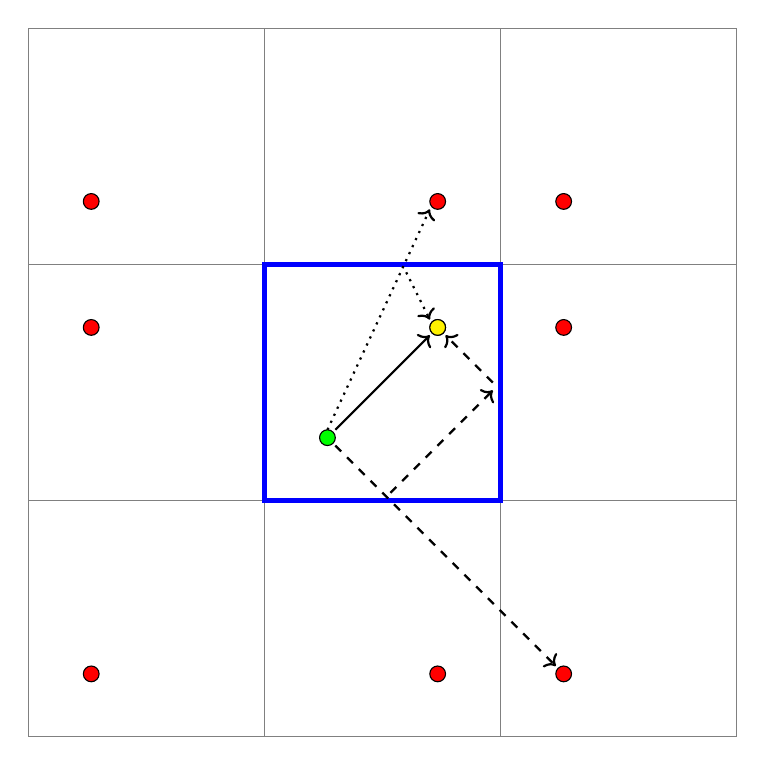
\begin{tikzpicture}[node distance = 5cm, auto]
	% grid
	\draw[step=3cm,gray,thin] (0,0) grid (9,9);
	\draw[draw=blue,ultra thick] (3,3) rectangle (6,6);

	% transmitter
	\filldraw[fill=green] (3.8,3.8) circle (1mm);
	% receiver replicas
	\foreach \x in {0.8,5.2,6.8}
		\foreach \y in {0.8,5.2,6.8}
			\filldraw[fill=red] (\x,\y) circle (1mm);
	% receiver
	\filldraw[fill=yellow] (5.2,5.2) circle (1mm);

	% lines
	% straight
	\draw[thick,->,draw=black] (3.9,3.9) -- (5.1,5.1); 
	% one reflection
	% \draw[thick,->,draw=black,dotted] (3.6,3.9) -- (0.9,5.1);
	% \draw[thick,->,draw=black,dotted] (3.1,4.2) -- (5.1,5.1);
	% one reflection
	\draw[thick,->,draw=black,dotted] (3.8,3.9) -- (5.1,6.7);
	\draw[thick,->,draw=black,dotted] (4.8,5.9) -- (5.1,5.3);
	% two reflections
	\draw[thick,->,draw=black,dashed] (3.9,3.7) -- (6.7,0.9);
	\draw[thick,->,draw=black,dashed] (4.6,3.1) -- (5.9,4.4);
	\draw[thick,->,draw=black,dashed] (5.9,4.5) -- (5.3,5.1);

\end{tikzpicture}
	\caption{Some possible reflections}
	\label{fig:rep1-reflections-ill}
\end{figure}

Given a square room, confined by the blue lines in Figure~\ref{fig:rep1-reflections-ill}, with a sound source depicted by the green dot and a microphone depicted by the yellow dot, it is easy to calculate the number of reflections heard at the yellow dot by mirroring the room about each wall. If the number of reflections is one, the result is that each wall must be mirrored once and the result is figure \ref{fig:rep1-reflections-ill} excluding the four corner rooms, for a total of five reflections (no reflection + 4 reflections). The red dots in the reflected rooms represent the yellow dot as projected through the wall (mirrored). After 2 reflections, Figure~\ref{fig:rep1-reflections-ill} should be extended by four more rooms (on the left and right and above and under the current square), yielding a total of 13 possible reflections.

% To see the impulse response of the room with two reflections we made use of the \texttt{MATLAB} script provided in Appendix~\ref{appsec:sourcecode-reflections} The impulse response is shown in Figure~\ref{fig:reflections-impulse}.

We created a \texttt{MATLAB} model for the above situation with the amount of reflections (rooms) as parameter. This script makes use of the previously discussed mirroring-principle, along with the given equation for sound dampening in the medium $\alpha(r) = \frac{\beta}{r^2}$ \cite[91]{epo4-manual}. A resulting impulse response as well as the behavior for a rectangular pulse, for $\beta = 1$ and 2 reflections, are shown in Figure~\ref{fig:rep1-reflections-matlab}.

\begin{figure}[H]
	\centering
	\begin{subfigure}{0.49\textwidth}
		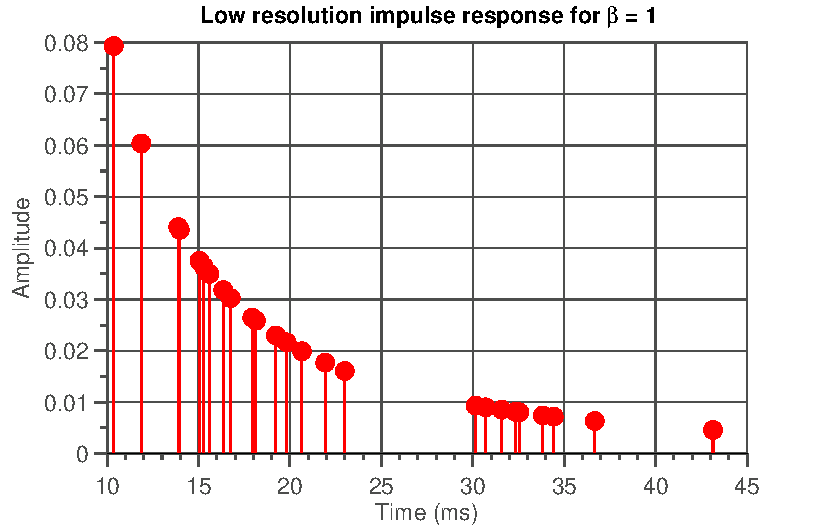
\includegraphics[width=\textwidth]{../../deliverable-7-resources/figures/ass-1/report-1/ass-1-report-1-impulse-response-2-copies-beta-1.pdf}
	\end{subfigure}
	\begin{subfigure}{0.49\textwidth}
		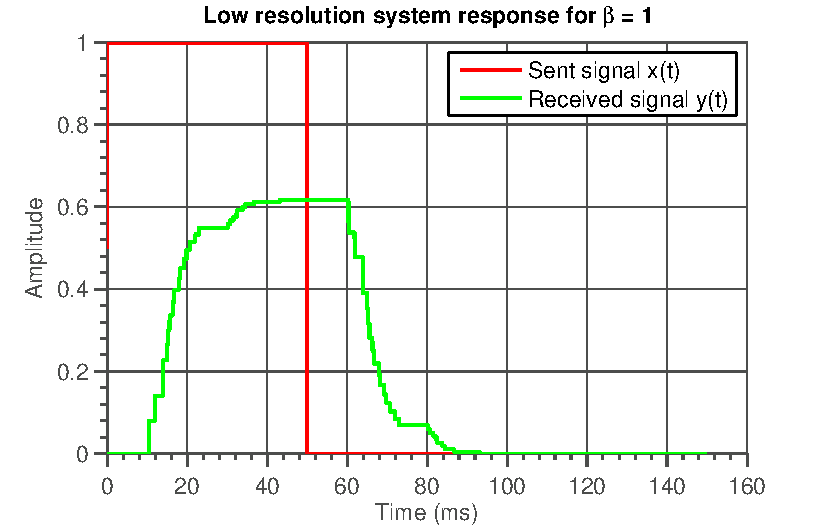
\includegraphics[width=\textwidth]{../../deliverable-7-resources/figures/ass-1/report-1/ass-1-report-1-system-response-2-copies-beta-1.pdf}
	\end{subfigure}
	\caption{Some possible reflections}
	\label{fig:rep1-reflections-matlab}
\end{figure}

\subsection{Report 2}
%corresponding matlab file: resource/labday1/report2.m
The impulse responses for a first order IIR filter $H(z) = \frac{1}{1+az^{-1}}$, with $a=0.95$ and $a=-0.95$ are shown in Figure~\ref{fig:rep2-time-resp}. For $a=0.95$ the filter causes a damped oscillation, for $a=-0.95$ it causes an exponentially decaying signal. Being a low-pass filter, the response for more general signals, will be a `smoothed' version of the original signal, since low-pass filters counteract rapid change in their input signals. % TODO, CHECK THIS

\begin{figure}[H]
	\centering
	\begin{subfigure}{0.49\textwidth}
		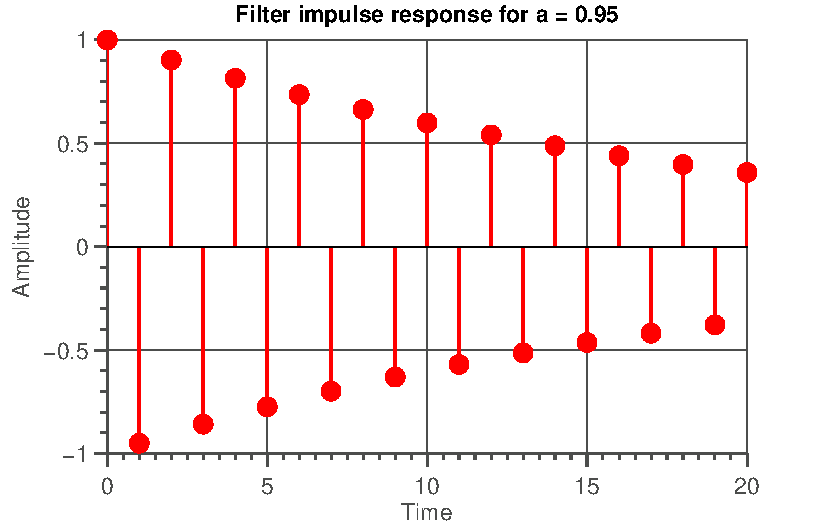
\includegraphics[width=\textwidth]{../../deliverable-7-resources/figures/ass-1/report-2/ass-1-report-2-a-positive.pdf}
	\end{subfigure}
	\begin{subfigure}{0.49\textwidth}
		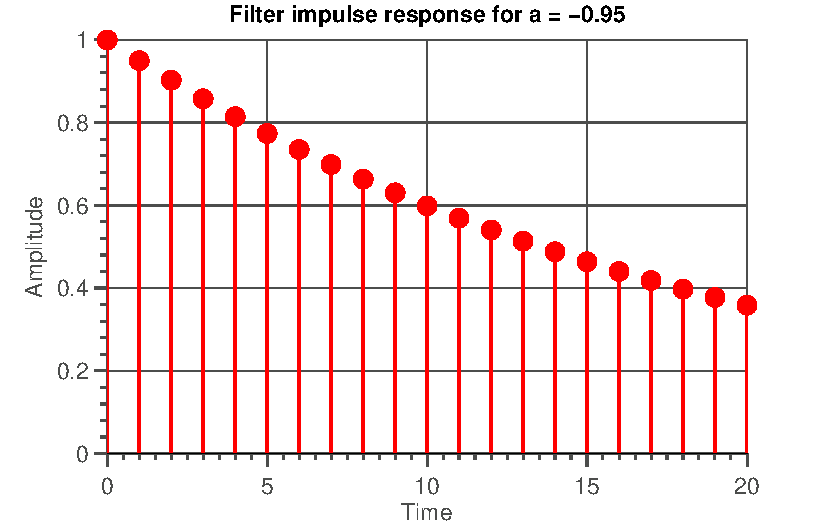
\includegraphics[width=\textwidth]{../../deliverable-7-resources/figures/ass-1/report-2/ass-1-report-2-a-negative.pdf}
	\end{subfigure}
	\caption{Impulse response of the given filter for two values of $a$}
	\label{fig:rep2-time-resp}
\end{figure}

The frequency impulse spectra are shown in Figure~\ref{fig:rep2-freq-resp}. It can be seen that for $a=0.95$ the filter behaves as a band pass filter and for $a=-0.95$ it behaves as a band stop filter. %INCORRECT, TODO: FIX THIS

\begin{figure}[H]
	\centering
	\begin{subfigure}{0.49\textwidth}
		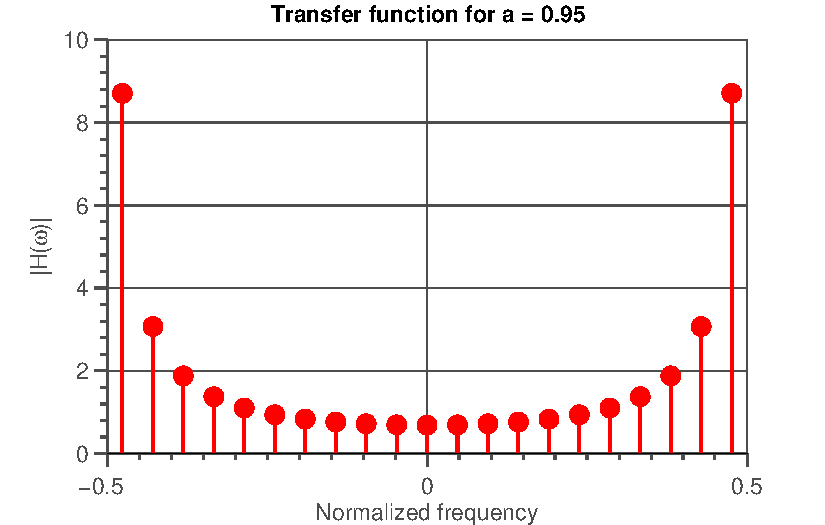
\includegraphics[width=\textwidth]{../../deliverable-7-resources/figures/ass-1/report-2/ass-1-report-2-a-positive-spectrum.pdf}
	\end{subfigure}
	\begin{subfigure}{0.49\textwidth}
		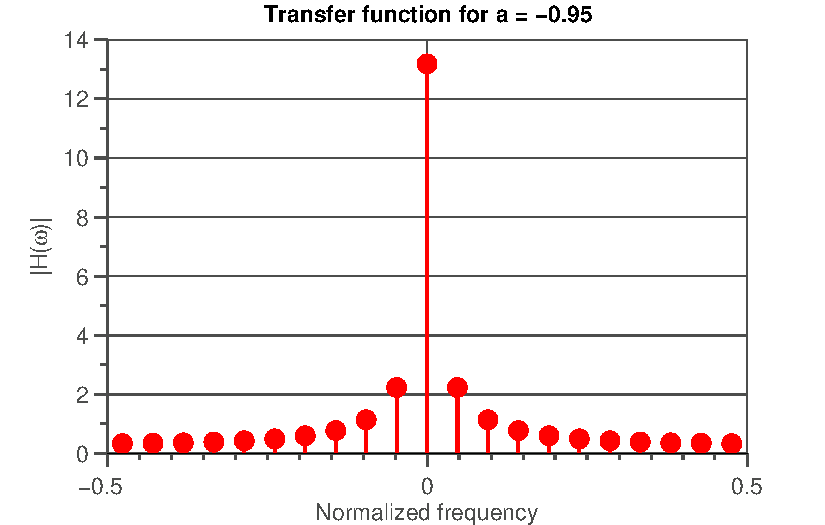
\includegraphics[width=\textwidth]{../../deliverable-7-resources/figures/ass-1/report-2/ass-1-report-2-a-negative-spectrum.pdf}
	\end{subfigure}
	\caption{The frequency response of the given filter for two values of $a$}
	\label{fig:rep2-freq-resp}
\end{figure}

There is no \texttt{MATLAB} function for the FT or DTFT, because a digital computer system and its software (like \texttt{MATLAB}) by definition cannot handle non-discrete signals, both amplitude and time need to be discrete. Since the FT and DTFT both have (partially) non-discrete in- and outputs, it is not possible to perform such calculations on a computer.

\subsection{Report 3}

\begin{figure}[H]
	\centering
	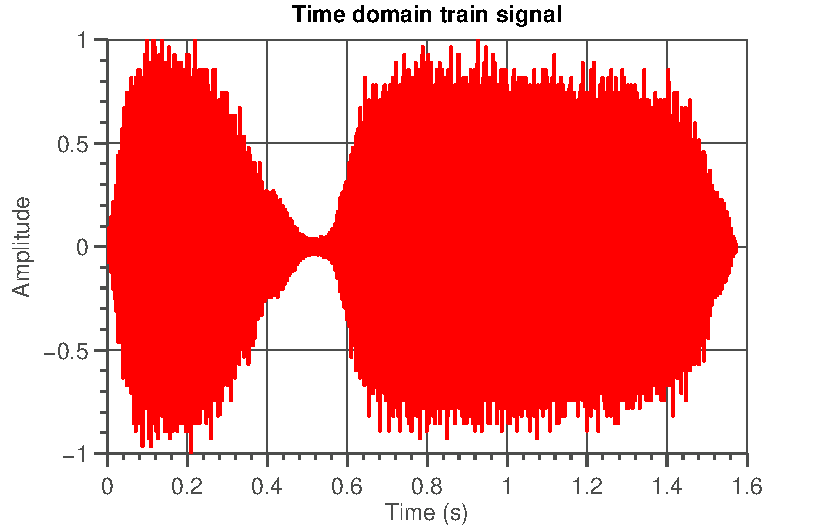
\includegraphics[width=0.6\textwidth]{../../deliverable-7-resources/figures/ass-1/report-3/ass-1-report-3.pdf}
	\caption{The time-domain signal of \texttt{MATLAB}'s train}
	\label{fig:rep3-train-time}
\end{figure}

A plot of the time-domain signal is given in Figure~\ref{fig:rep3-train-time}, we can distinguish the two whistle blows (`woo-wooooo'), but otherwise there is not much more that can be said about it.

\subsection{Report 4}
%Corresponding matlab file: resources/labday1/report4.m
Figure~\ref{fig:rep4-train-heatmap} shows a heatmap of the occurrence of frequencies in \SI{20}{\milli\second} intervals of \texttt{MATLAB}'s train audio signal. This plot should give a more detailed view of the frequency contents of the train signal than a normal signal spectrum would, since it also includes a time component. It is apparent that most of the sound is centered around \SI{3}{\kilo\hertz}. The two whistle blows are also clearly distinguishable.

\begin{figure}[H]
	\centering
	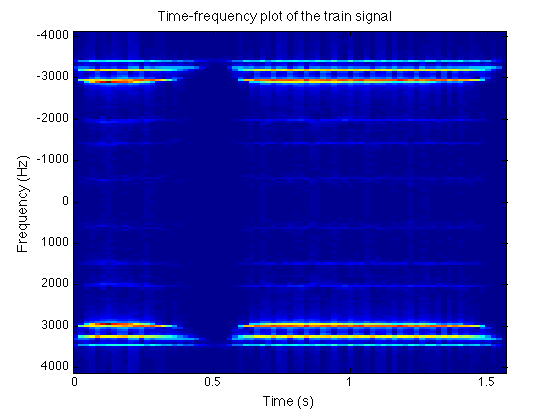
\includegraphics[width=0.6\textwidth]{../../deliverable-7-resources/figures/ass-1/report-4/ass-1-report-4.png}
	\caption{The frequency-time heatmap of \texttt{MATLAB}'s train}
	\label{fig:rep4-train-heatmap}
\end{figure}

\subsection{Report 5 and 6}

\begin{figure}[H]
	\centering
	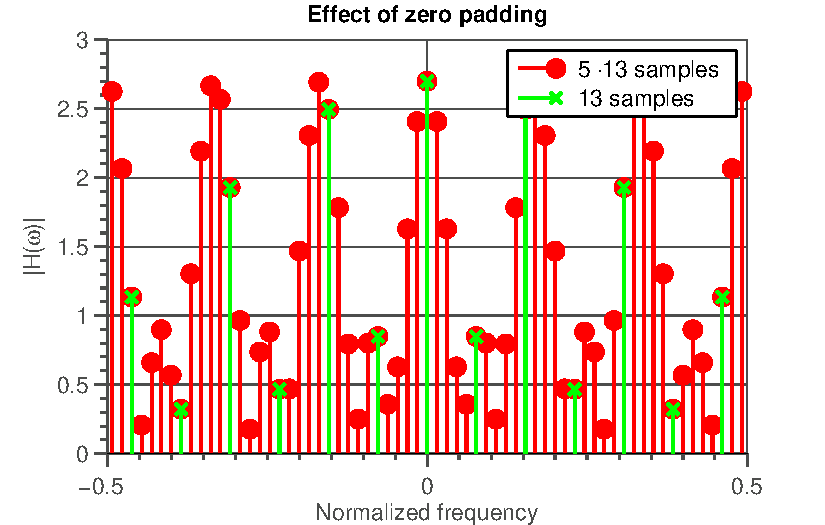
\includegraphics[width=0.6\textwidth]{../../deliverable-7-resources/figures/ass-1/report-5-6/ass-1-report-5-6.pdf}
	\caption{The frequency spectrum of the given signal $a$, with and without zero padding, obtained using FFT}
	\label{fig:rep5-6-spectrum}
\end{figure}

Figure~\ref{fig:rep5-6-spectrum} shows the frequency spectrum of the original given $h$ after FFT, as well as a padded $h$ which is five times longer than the original. Comparing the plots, we see that interpolation is indeed accomplished, just be adding zeros to the end of our original signal. Since our padded $h$ is five times larger than the original, we notice that every 5th sample in the padded response indeed coincides with a sample of the original one.

\subsection{Report 7}

\begin{figure}[H]
	\centering
	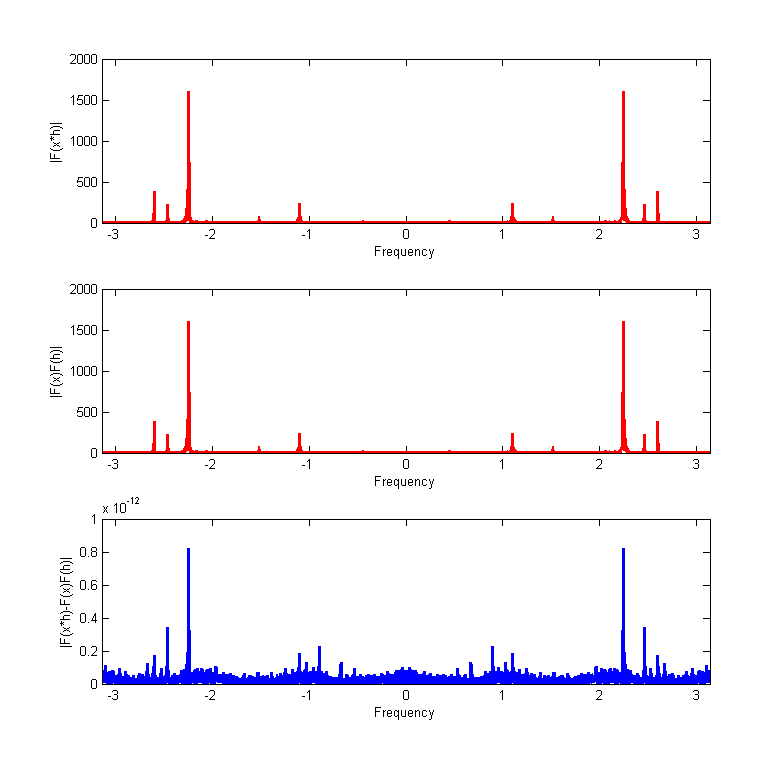
\includegraphics[width=0.8\linewidth]{../../deliverable-7-resources/figures/ass-1/report-7/ass-1-report-7-temp.png}
	\caption{Amplitude spectra for convolving first then FFT, FFT first then multiplying and the absolute difference between the methods.}
	\label{fig:rep7}
\end{figure}

To test whether the convolution property holds, the `train' signal was convolved with the same, extended $h[n]$ as before. The result was then FFT'd and the amplitude spectrum was drawn. Then, for the same `train' signal and $h[n]$ these signals were first FFT'd and then multiplied. Again, an amplitude spectrum was plotted. The results of both these plots can be found in Figure~\ref{fig:rep7}, along with a third plot, the absolute difference between the two results. We may conclude that first convolving and then applying an FFT yields almost the same results as first applying an FFT and then multiplying. The differences are in the order of $10^{-13}$ to $10^{-12}$, which we can attribute to numerical and round-off errors in the FFT implementation and convolution algorithms.
\end{document}